\doublespacing

In the previous chapter, we developed a systematic method for constructing effective real space potentials that incorporate realistic effects into Monte Carlo (MC) simulations of the fractional quantum Hall effect (FQHE). In this chapter, we apply our method to the effect of Landau level mixing (LLM) in the lowest Landau level (LLL) of graphene. We calculate the composite fermion (CF)-exciton dispersion via MC and benchmark the results against an exact calculation via exact diagonalization.

\section{Composite Fermion-Exciton Dispersion for Small Systems} \label{sec:enGaps}

    \subsection{Exact Diagonalization} \label{ssec:exDi}
    In order to benchmark the MC calculations, which are approximate by nature, we can calculate the exciton disperson exactly for small systems ($N\lesssim 10$).  Since this thesis focuses mostly on constructing real space potentials describing realistic effects for use in MC calculations, we will only briefly outline how the exact calculations are done. 
    
    The CF wavefunction for electron filling factor $\nu=1/3$ is equivalent to the Laughlin wavefunction. It turns out that this state can be written as an exact expansion of Slater determinants (basis states) by exactly diagonalizing the so-called ``hard core", or ``$V_1=\infty$", potential~\cite{haldane}. Practically, this means we set the ratio of $V_1/V_m\rightarrow\infty$ for all $m\neq 1$. This amounts to exactly diagonalizing the Hamiltonian in Eq.~\ref{HamPPexpand} with $V_m/V_1=0$ for all $m\neq 1$. In the spherical geometry, in which we work, this translates to setting $V_{Q,Q}(L)/V_{Q,Q}(2Q-1)=0$ for all $L\neq 2Q -1$. The Laughlin state $|\Psi_{1/3}(L=0)\rangle$ is the zero energy ground state of the aforementioned Hamiltonian. We can also find the low energy branch of excitations for calculating the exciton dispersion (see Sec.~\ref{sec:compFerm}) by diagonalizing the ``hard-core" potential $|\Psi_{1/3}(L)\rangle$. 
    
    Given the Haldane pseudopotentials (PPs) of a realistic FQH state (e.g. graphene on a substrate), we can insert Eq.~\ref{potLlm} into Eq.~\ref{HamPPexpand} to construct the Hamiltion as
    \begin{eqnarray}
    H_\mathrm{realistic} = \sum_m (V_m^{(0)} + \kappa \delta V_m^{(0)})\sum_{i<j} P_{ij}(m),
    \end{eqnarray}
    where the PPs are calculated using the single-particle basis states making up the Slater determinants. Now we can exactly calculate the exciton dispersion for $\nu=1/3$ by calculating the expectation value
    \begin{eqnarray}
    \frac{\langle \Psi_{1/3}(L)|H_\mathrm{realistic}|\Psi_{1/3}(L)\rangle}{\langle \Psi_{1/3}(L)|\Psi_{1/3}(L)\rangle}\;.
    \end{eqnarray}
    
    In the next section, we use these exact calculations to benchmark the MC exciton dispersion for $6\leq N\leq10$ electrons with LLM parameter $\kappa\in\{0.0,0.1,0.2\}$.

\iffalse    
    In this section, we will briefly sketch the method for which the CF ground state and low-energy excitation eigensystem can be obtained via exact diagonalization following from Appendix L of Ref. \cite{jain}.
    
    To diagonalize the Hamiltonian matrix, we must orthogonalize the CF basis functions of LLL projected wave functions via the Gram–Schmid procedure. We begin with the normalized states
    
    \begin{equation}\label{normStat}
    \left|\eta_{\alpha}\right\rangle \equiv \frac{\left|\Psi_{\alpha}\right\rangle}{\sqrt{\left\langle\Psi_{\alpha} \mid \Psi_{\alpha}\right\rangle}},
    \end{equation}
    
    with scalar products $\mathcal{O}_{\alpha \beta} \equiv\left\langle\eta_{\alpha} \mid \eta_{\beta}\right\rangle$. We can find the orthogonal basis states 
    
    \begin{equation}\label{orthBasStat}
    \left|\xi_{\alpha}\right\rangle\equiv \sum_{\beta} U_{\alpha \beta}|\eta \beta\rangle=\left|\eta_{\alpha}\right\rangle-\sum_{\gamma=1} \frac{\left\langle\xi_{\gamma} \mid \eta_{\alpha}\right\rangle}{\left\langle\xi_{\gamma} \mid \xi_{\gamma}\right\rangle}\left|\xi_{\gamma}\right\rangle,
    \end{equation}
    
    where the transformation matrix $U_{\alpha \beta}$ is given by the recursion relation
    
    \begin{equation}
    U_{\alpha \beta}=\left\{\begin{array}{cc}
    -\sum_{\gamma=1}^{\alpha-1} \frac{\sum_{\delta=1}^{\gamma} U_{\gamma \delta}^{*} \mathcal{O}_{\delta \alpha}}{\sum_{\delta, \epsilon=1}^{\gamma} U_{\gamma \delta}^{*} U_{\gamma \epsilon} \mathcal{O}_{\delta \epsilon}} U_{\gamma \beta} & \text { for } \beta<\alpha \\
    1 & \text { for } \beta=\alpha, \\
    0 & \text { for } \beta>\alpha.
    \end{array}\right.
    \end{equation}
    
    We can obtain the CF energy
    \begin{equation}
    V_{\alpha \beta}=\frac{\left\langle\xi_{\alpha}|V| \xi_{\beta}\right\rangle}{\sqrt{\left(\xi _ { \alpha } | \xi _ { \alpha } \rangle \left(\xi_{\beta}\left|\xi_{\beta}\right\rangle\right.\right.}},
    \end{equation}
    where $\left\langle\xi_{\alpha}|V| \xi_{\beta}\right\rangle &=\sum_{\gamma, \delta} U_{\alpha \gamma}^{*} U_{\beta \delta}\left\langle\eta_{\gamma}|V| \eta_{\delta}\right\rangle$ and $\left\langle\xi_{\alpha} \mid \xi_{\alpha}\right\rangle &=\sum_{\gamma, \delta} U_{\alpha \gamma}^{*} U_{\beta \delta} \mathcal{O}_{\gamma \delta}$.
    
    The exact diagonalization results that we are benchmarking the MC code results against for the ground state energies were done by Ryan Towne and the low energy excitations were done by by Michael R. Peterson. The ED code was executed with data we provided of the approximated LLM-incorporated PPs, so both the MC and ED codes use identical PPs for each state and therefore should return similar energies.
\fi
     
    \subsection{Benchmark Results} \label{ssec:benchmRes}
    
    The MC code is written in the \texttt{C} programming language and is implemented in parallel via the library \texttt{Open MPI}. The code's execution was distributed among ten cores of the California State University Long Beach central High Performance Computing (HPC) cluster, and the following benchmarks took on the order of tens of minutes to run (in total). The MC standard error is calculated by dividing the trials into ten groups of one million consecutive iterations, and then calculating the variance between the groups as discussed in Sec. \ref{sec:enExpVal}. In Fig.~\ref{fig:exc_disp_ns}, we break down the contribution to the low energy exciton dispersion from each system size within our benchmarks ($6\leq N\leq10$) as a function of the wave vector $kl=L/\sqrt{Q}$ for the bare Coulomb potential in the LLL. As the system size increases, the dispersion converges to one solid line, which converges to the transport gap $\Delta_t$ at large wave vectors. 
  
   \begin{figure}[H]
    \begin{center}
    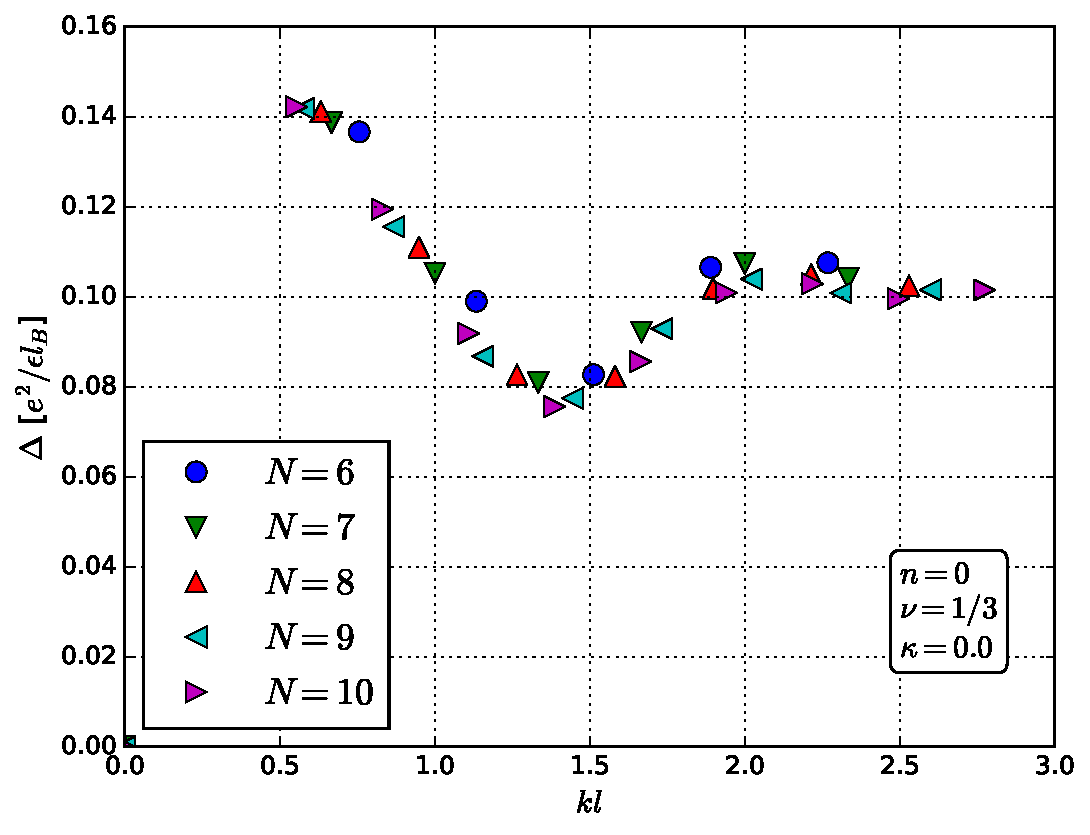
\includegraphics[width=10cm, angle=0]{ThesisCSULBLatexTemplate/figures/exc_disp_ns.pdf}
    \caption[The low energy CF-exciton dispersion broken down by system size.]{The low energy CF-exciton dispersion broken down by system size. We plot the exciton dispersion $\Delta$ for the bare Coulomb potential (LLM parameter $\kappa=0.0$) as a function of the wave vector $kl$ as calculated by the MC code for $6\leq N\leq10$ electrons at filling factor $\nu=1/3$ in the LLL ($n=0$).}
    \label{fig:exc_disp_ns} 
    \end{center}
    \end{figure}
    
    In Fig.~\ref{fig:exc_disp_kappas}, we plot the exciton dispersions produced by both MC and exact diagonalization for the benchmarks $6\leq N\leq10$ and $\kappa\in\{0.0,0.1,0.2\}$. As a general trend, the exciton dispersion shifts vertically downwards as a function of increasing $\kappa$ when calculated by exact diagonalization. This is expected since LLM effects reduce Haldane pseudopotentials (PPs) systematically and are expected to reduce all energies and energy gaps (see Sec.~\ref{ssec:apprEffPot}). The opposite trend, however, is observed when calculating the exciton dispersion via MC. The difference between these two trends is easier to see in Fig. \ref{fig:transp_gaps_vs_kappa}, where we plot just the transport gaps (calculated as the gap from the ground state energy to the lowest energy at the maximum total angular momentum state $L_{max}=N$) as a function of $\kappa$. The MC transport gaps increase with increasing $\kappa$, while the exact diagonalization benchmarks decrease with increasing $\kappa$. In the next section we discuss the sources of this error.
    
    \begin{figure}[H]
    \begin{center}
    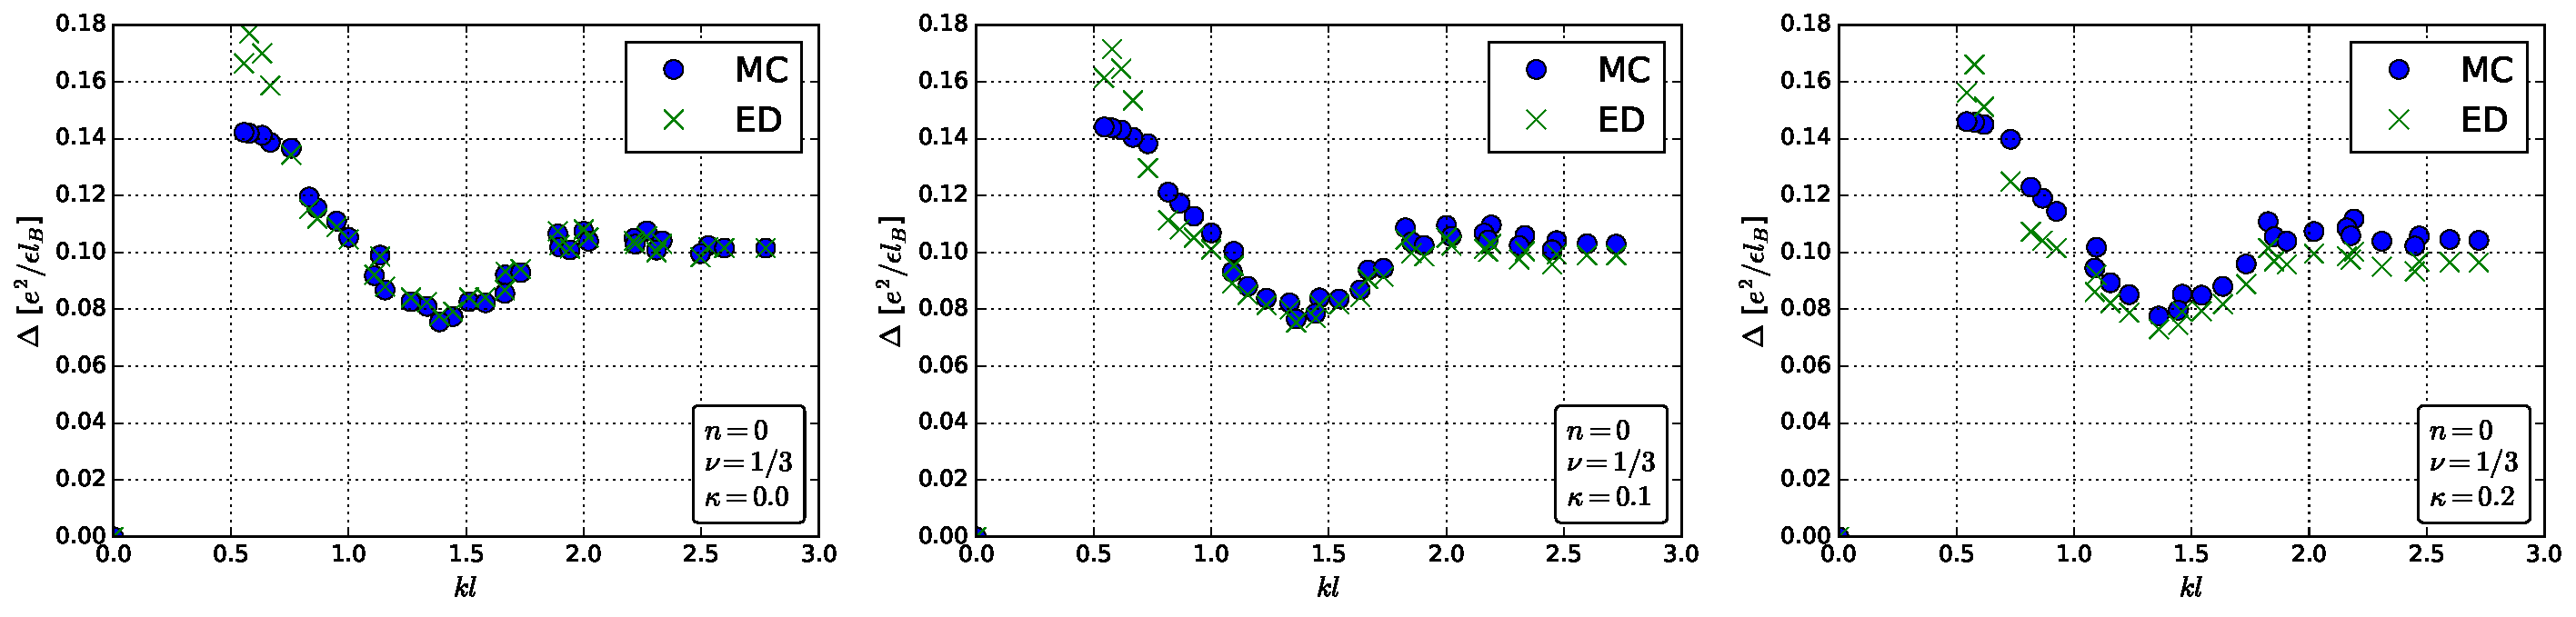
\includegraphics[width=10cm, angle=0,scale=1.5]{ThesisCSULBLatexTemplate/figures/exc_disp_kappas.pdf}
    \caption[The exciton dispersion benchmarks for different values of the LLM parameter.]{The exciton dispersion benchmarks for different values of the LLM parameter. The exciton ($\Delta$) dispersion as calculated by Monte Carlo (MC) and the exact diagonalization (ED) benchmarks is plotted as a function of the wave vector $kl$ in the LLL ($n=0$) for electron filling factor $\nu=1/3$ and $\kappa\in\{0.0,0.1,0.2\}$.}
    \label{fig:exc_disp_kappas} 
    \end{center}
    \end{figure}
    
    \begin{figure}[H]
    \begin{center}
    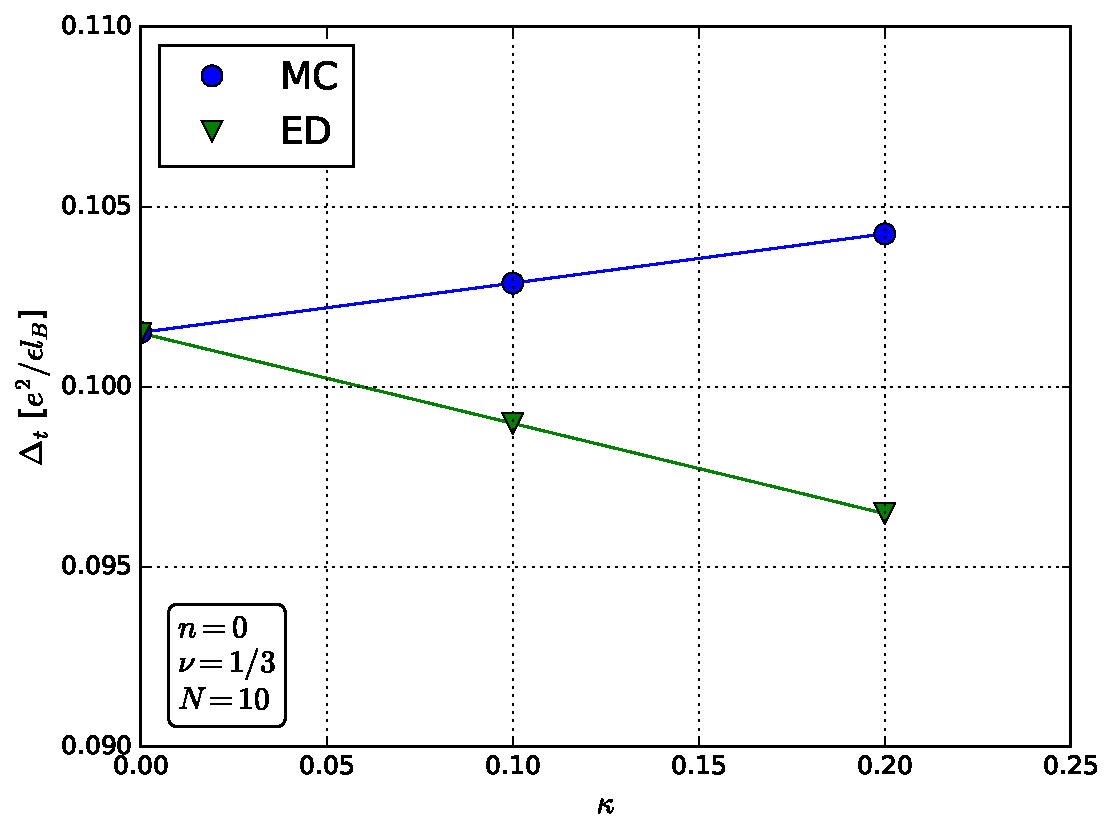
\includegraphics[width=10cm, angle=0]{ThesisCSULBLatexTemplate/figures/transp_gaps_vs_kappa.pdf}
    \caption[The transport gap benchmarks as a function of the LLM parameter.]{The transport gap benchmarks as a function of the LLM parameter. The constant approached at large wave vectors for a far separated CF-quasiparticle and CF-quasihole pair (transport gap $\Delta_t$) is plotted for $N=10$ electrons as a function of the LLM parameter $0.0\leq\kappa\leq0.2$ for Monte Carlo (MC) and the exact diagonalization (ED) benchmarks at filling factor $\nu=1/3$ in the LLL ($n=0$).}
    \label{fig:transp_gaps_vs_kappa}
    \end{center}
    \end{figure}
    
    \subsection{Sources of Error} \label{ssec:sourcErr}
    
    In the previous section, we used our method to calculate an exciton dispersion via MC and observed it had the opposite trend of the benchmark. We seek to explain this discrepancy in this section. In Fig. \ref{fig:transp_gaps_vs_kappa}, the MC transport gap matched comparatively well with the exact diagonalization transport gap for the bare Coulomb potential ($\kappa=0$). It then shifted vertically upward as $\kappa$ increased, in opposition to the benchmark. We believe this can be explained by looking at the configurations of electrons on the surface of the Haldane sphere which were accepted by the Metropolis-Hastings algorithm. 
    
    As mentioned in Secs.~\ref{ssec:montCarlInt} and~\ref{ssec:compFerm}, we start the MC code with electrons in a random configuration on the sphere, perturb each electron slightly in a random direction, and then calculate whether it is more likely to be in the perturbed (trial) configuration or the previous one. As mentioned in Sec.~\ref{ssec:compFermExcDisp}, we use the wavefunction for the lowest energy state at maximum total angular momentum ($L_{max}=N$) to calculate the probability of being in the trial or previous configuration. This means that if we were to plot a histogram representing the probability of each possible configuration getting accepted by the Metropolis-Hasting algorithm, it should closely resemble the pair correlation function of the CF wavefunction itself. This is designed so that the average energy of our accepted configurations (Eq.~\ref{metrAppr}, where $\mathcal{O}(\mathbf{R}^{(n)})=\sum_{i<j}V(|\mathbf{r}_i-\mathbf{r}_j|)$) quickly converges to the corresponding energy expectation value (Eq.~\ref{cfInt}) by sampling from the most likely states. 
    
    On the right side of Fig.~\ref{fig:r_sample_hist}, we plot a histogram representing the likelihood of each chord distance between two electrons on the sphere ($r=|\mathbf{r}_i-\mathbf{r}_j|$) being found in a configuration that was accepted by the Metropolis-Hastings algorithm. We can see in the figure that the distribution of the accepted distances has a strong negative skew. In other words, it does not represent a symmetric Gaussian distribution - the peak probability is skewed towards the larger values of $r$. This means that the CF wavefunction wants to, for the most part, keep the electrons as far away from each other as possible while still remaining on the sphere's surface. This behavior is expected since the wavefunction seeks to minimize the Coulomb energy of the electrons, which decreases as a function of their separation distance.
    
    On the left side of Fig.~\ref{fig:r_sample_hist}, we plot the difference between the effective real space potential and the bare Coulomb potential, $V_{eff}-V_{Coul}$ (see Sec.~\ref{ssec:apprEffPot}). This reflects the changes made to the Coulomb potential when incorporating LLM. We can see in the figure that at very small distances LLM decreases the potential, at mid-range distances it slightly increases it, and at far distances it has little to no effect. According to the histogram on the right side of the figure, the configurations where electrons are closer together, where LLM most affects the potential, are seldom accepted by the Metropolis-Hastings algorithm. It overwhelmingly samples from configurations where the particles are as far apart as possible and the Coulomb potential is mostly unchanged. To add to this, it samples more from the region of the histogram where $V_{eff}>V_{Coul}$ than it does from the region where $V_{eff}<V_{Coul}$, which explains why the transport gaps increase in the MC code with increasing $\kappa$ (please see Appendix~\hyperref[appendixB]{B} for more details on the behavior of the effective potential in real space).
    
    \begin{figure}[h]
    \begin{center}
    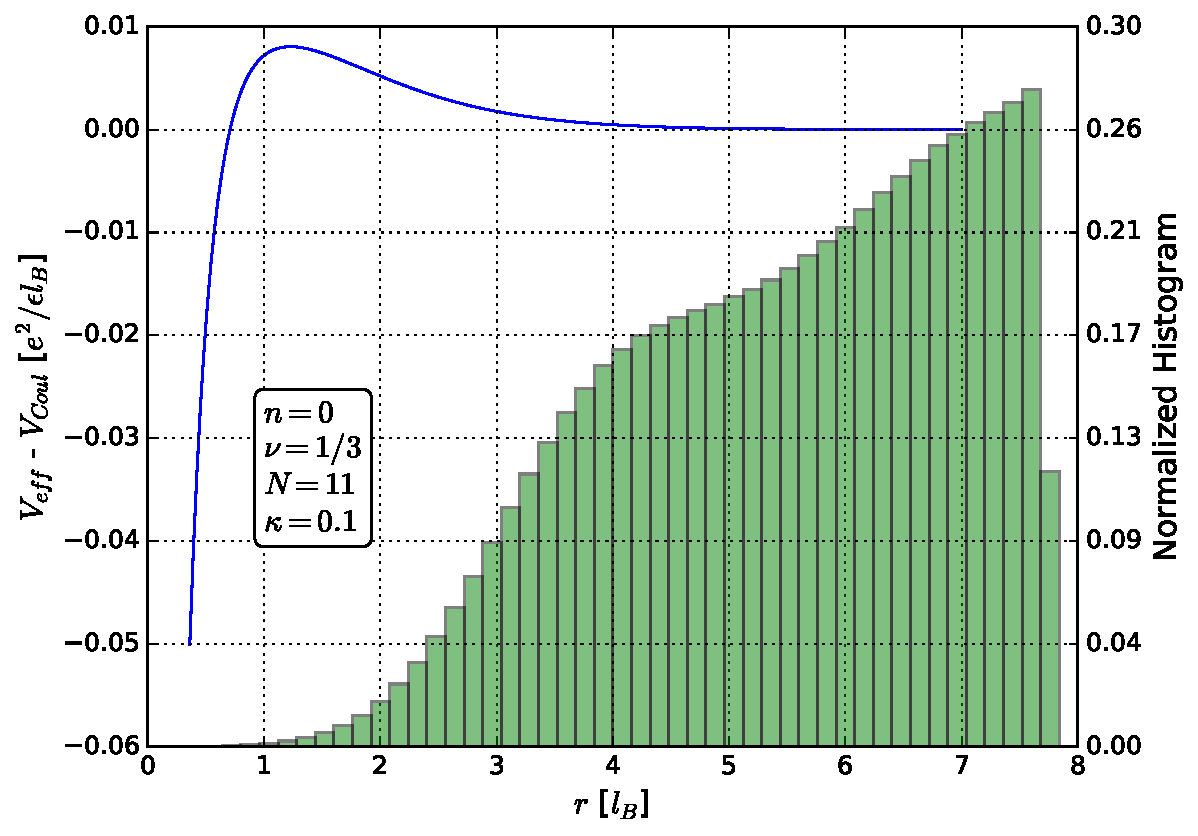
\includegraphics[width=10cm, angle=0]{ThesisCSULBLatexTemplate/figures/r_sample_hist.pdf}
    \caption[The potential difference due to LLM compared to the electron configurations accepted by the Metropolis-Hastings algorithm.]{The potential difference due to LLM compared to the electron configurations accepted by the Metropolis-Hastings algorithm. On the left vertical axis, we plot the difference between the LLM-incorporated modified Park potential and bare Coulomb potential $V_{eff}-V_{Coul}$ in real space as a function of the chord distance $r$ between electrons on the surface of the Haldane sphere. On the right vertical axis, we plot a normalized histogram showing the likelihood of a configuration with a chord distance $r$ being accepted by the Metropolis-Hastings algorithm. LLM most affects the configurations where electrons are closest together, but these are seldom accepted by the Metropolis-Hastings algorithm. This trial was done in the LLL ($n=0$) at filling factor $\nu=1/3$ for $N=11$ electrons and LLM parameter $\kappa=0.1$.}
    \label{fig:r_sample_hist} 
    \end{center}
    \end{figure}
    
    Several attempts were made to alleviate this systematic error. For our benchmarks, the radius of the Haldane sphere is fixed at $R=\sqrt{Q}l_B$ (see Sec.~\ref{sec:haldPseud}) with magnetic monopole strength $Q=3/2(N-1)$ (see Sec.~\ref{ssec:apprEffPotPar}). We cannot then, for example, bring the electrons closer together by decreasing the sphere's radius. Adding more electrons correspondingly increases the radius and spaces them out more. Increasing the number of iterations up to $10^9$ (as mentioned in Sec. \ref{sec:enExpVal}) made no significant difference to the accuracy of our simulations. We looked for a trend in the transport gap as a function of the number of iterations but this was not conclusive as the differences between trials with increased numbers of iterations were less than the standard error, which was comparatively very small. We also tried fine-tuning the ratio $\eta$, which determines whether a configuration will be accepted (see Sec.~\ref{ssec:compFerm}), to a constant value, but this did not provide consistent results across different systems. 
    
    We were inspired to try a technique called Laplace smoothing which is used to alleviate the zero frequency problem in the Naive Bayes model of machine learning \cite{kikuchi}. The idea behind our application of this was to artificially add an extra distance $r$ to each radius bin of the histogram so that the smallest radii were sampled $>0$ times while still trying to preserve the relative likelihood of the distances being sampled. In practice, we attempted this through multiple different initial conditions and behaviors for a variable number of pre-Metropolis-Hastings algorithm iterations. One example was starting with the electrons arranged in a circle very close to the north pole of the sphere, then accepting each configuration as they slowly moved down towards the equator before beginning the algorithm. We also tried starting with the electrons bunched close together on a line at the equator, accepting each step as they slowly spread out along the equator, and then starting the algorithm. We believe these methods produced large errors because we artificially inserted too many highly improbable states at too high of a frequency for the MC average energy to quickly converge to the energy expectation value.
    
    We were also inspired by work with quantum annealing \cite{finnila}. We tried implementing a parameter that described the number of MC iterations before a thermal fluctuation would reset the system to a random state. We believe that this method did not make any significant changes to our results because in practice the Metropolis-Hastings algorithm ended up being so good at finding equilibrium that it too quickly bypassed the less likely states where LLM was most affecting the real space potential. After adjusting every parameter in the MC code we could think of, we became closely acquainted with how sensitive our implementation of the Metropolis-Hastings algorithm is to changes made by the user. We conclude that the algorithm itself is not amenable to changes to which configurations are accepted, and therefore suggest further study be done to develop a new algorithm that can efficiently sample the configurations where realistic effects most change the real space potential so that MC estimates of FQH energies can be calculated in better agreement with experimental data collected in environments where effects often overlooked by theorists cannot be quenched.

\singlespacing